\subsection{GUI}

På figur \ref{PAA}, kan det ses hvordan, det var muligt at sende kommandoen 5 ved at bruge ”Planlæg åbning” funktionen. 

\begin{figure}[H]
	\includegraphics[scale=1]{tex/Test/GUI-Test/Billeder/test_GUI}
	\caption{Åben nu funktionen implementerets}
	\label{PAA}
\end{figure}

På figur \ref{PAA} ses hvordan GUI meddeler 
bruger statusbeskeder på baggrund af den kommando som blev indlæst fra txt filen.

\begin{figure}[H]
	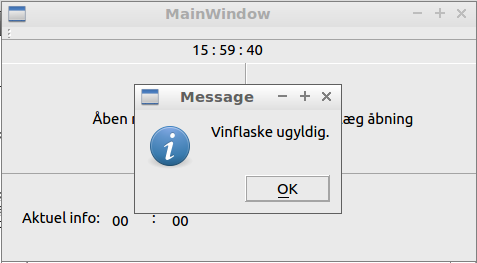
\includegraphics[scale=1]{tex/Test/GUI-Test/Billeder/Test_Virtuel_klasse_invalid}
	\caption{Test at virtuel klasse}
	\label{PAA}
\end{figure}